\subsection*{Grey Box Sequence Diagram}
\begin{figure}[H]
	\centering
	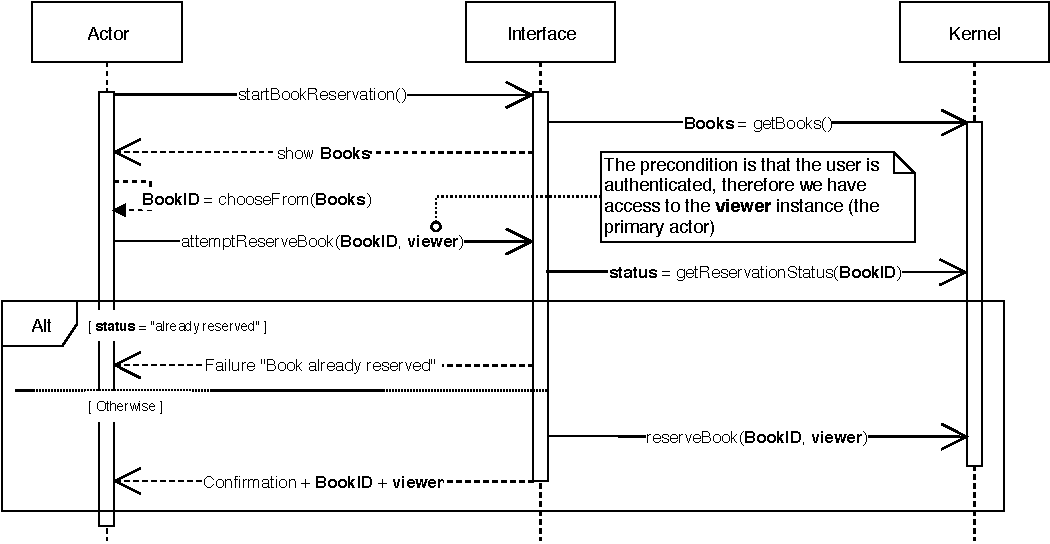
\includegraphics[scale=.9]{uml/SD-gb-reserve.pdf}
	\caption*{Grey Box diagram for use case C2, made by A}
\end{figure}
The interface in a grey box acts as an intermediate step between the actor and the kernel. User commands are passed to the interface, and it in turn can do some minor operations before delegating it to the kernel.\\For example, after starting the transaction, we need the actor to choose a book they want to have reserved. We ask the kernel to fetch the list of books and present it to the actor. The actor selects a book and provides it, along with their ID, which is accessable since the actor has been authenticated. Before delegating the reservation, we check whether the book has already been reserved, returning a failure if so. Otherwise we request the kernel to reserve the book and return a confirmation.
\subsection*{White Box Sequence Diagram}
\begin{figure}[H]
	\centering
	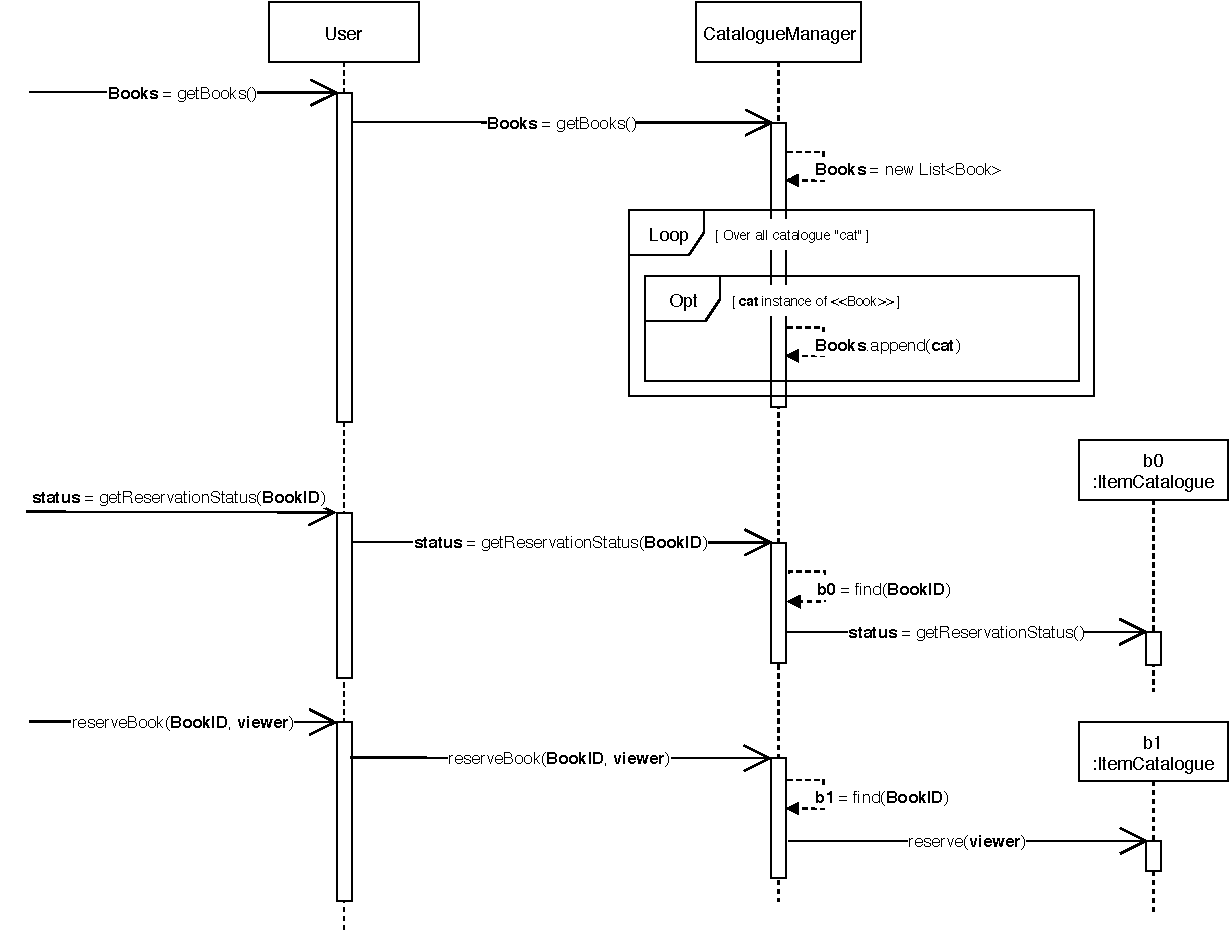
\includegraphics[scale=.80]{uml/SD-wb-reserve.pdf}
	\caption*{White Box diagram for use case C2, made by A}
\end{figure}
A white box sequence diagram offers a high level implementation of the requests going to the kernel in the gray box sequence diagram. In this case, the implementations are fairly straigtforward. For ``getBooks()'' we delegate the request to CatalogueManager which fetches all catalogues that are an instance of the Book class, since Book inherits ItemCatalogue. ``getReservationStatus(..)'' is checks all catalogues for the specific book they are looking for and returns its reservation status. Similarly, ``reverveBook(..)'' sets the reservation status.